\documentclass[12pt]{article}
\usepackage[ngerman]{babel}\usepackage[babel=true]{microtype}
\usepackage[utf8]{inputenc}
\usepackage[T1]{fontenc}\usepackage{lmodern}\usepackage{color}
\usepackage[a4paper,includeheadfoot,
top=2cm, 
bottom=2cm, 
left=2cm, 
right=2cm]{geometry}
\usepackage{listings}\usepackage{color}\usepackage{tikz}
\usepackage{amsmath,amssymb,amsfonts,amsthm}
\usepackage{graphicx} %\includegraphics[width=0.7\textwidth]{bild.jpg}
\usepackage{placeins} %for \FloatBarrier
\usepackage[colorlinks=false,pdfborder={0 0 0}]{hyperref}%Hide RED PDF Border
\usepackage{fancyhdr}\pagestyle{fancy}
\usepackage{xcolor} 
\definecolor{hintergrund}{HTML}{B0C4E3} \definecolor{cobalt}{rgb}{0.0, 0.28, 0.67}
\usepackage{sectsty} \sectionfont{\color{cobalt}} \subsectionfont{\color{cobalt}}
\usepackage[labelfont={normalfont,bf}, format=hang, justification=RaggedRight, singlelinecheck=false]{caption}

\lstset{literate=%Sonderzeichen in Listings
    {Ö}{{\"O}}1
    {Ä}{{\"A}}1
    {Ü}{{\"U}}1
    {ß}{{\ss}}1
    {ü}{{\"u}}1
    {ä}{{\"a}}1
    {ö}{{\"o}}1
    {~}{{\textasciitilde}}1
}
\definecolor{mygreen}{rgb}{0,0.6,0}
\definecolor{mygray}{rgb}{0.5,0.5,0.5}
\definecolor{mymauve}{rgb}{0.58,0,0.82}

\lstset{ %
  backgroundcolor=\color{white},   % choose the background color;
  basicstyle=\footnotesize,        % the size of the fonts that are used for the code
  breakatwhitespace=false,         % sets if automatic breaks should only happen at whitespace
  breaklines=true,                 % sets automatic line breaking
  captionpos=b,                    % sets the caption-position to bottom
  commentstyle=\color{mygreen},    % comment style
  deletekeywords={...},            % if you want to delete keywords from the given language
 % escapeinside={\%*}{*)},          % if you want to add LaTeX within your code
  extendedchars=true,              % lets you use non-ASCII characters; for 8-bits encodings only, does not work with UTF-8
  frame=single,	                   % adds a frame around the code
  keepspaces=true,                 % keeps spaces in text, useful for keeping indentation of code (possibly needs columns=flexible)
  keywordstyle=\color{blue},       % keyword style
  language=R,                 % the language of the code
  otherkeywords={*,...},           % if you want to add more keywords to the set
  numbers=left,                    % where to put the line-numbers; possible values are (none, left, right)
  numbersep=5pt,                   % how far the line-numbers are from the code
  numberstyle=\tiny\color{mygray}, % the style that is used for the line-numbers
  rulecolor=\color{black},         % if not set, the frame-color may be changed on line-breaks within not-black text (e.g. comments (green here))
  showspaces=false,                % show spaces everywhere adding particular underscores; it overrides 'showstringspaces'
  showstringspaces=false,          % underline spaces within strings only
  showtabs=false,                  % show tabs within strings adding particular underscores
  stepnumber=0,                    % the step between two line-numbers
  stringstyle=\color{mymauve},     % string literal style
  tabsize=2,	                   % sets default tabsize to 2 spaces
  title=\lstname                   % show the filename of files included with \lstinputlisting; also try caption instead of title
}

\addto\captionsngerman{%Abkürzen der Überschriften
\renewcommand{\figurename}{Schritt}
\renewcommand{\tablename}{Tab.}
}

\lstdefinestyle{base}{
  language=R,
  emptylines=1,
  breaklines=true,
  alsoletter={.},
  basicstyle=\ttfamily\color{blue},
  keywordstyle=\color{blue},
  moredelim=**[is][\color{red}]{@}{@},
}

\lhead{} \chead{Installation von \LaTeX~unter Windows} \rhead{Universität Bonn}
\lfoot{} \cfoot{\thepage} \rfoot{Stand: \today}

\begin{document}
\section*{Kurzanleitung:}
\begin{enumerate}
\item Lade TeX Live herunter
\item Starte den Installer und führe eine Vollinstallation durch
\item Installiere Texmaker
\item Sofern noch nicht vorhanden, installiere Adobe Acrobat Reader
\end{enumerate}


\section*{Schrittweise:}
%\begin{minipage}[t]{\textwidth}
\begin{figure}[h]
\centering
\captionof{figure}{Lade den Tex Live Installer hier herunter:\\ \url{http://mirror.ctan.org/systems/texlive/tlnet/install-tl-windows.exe}}
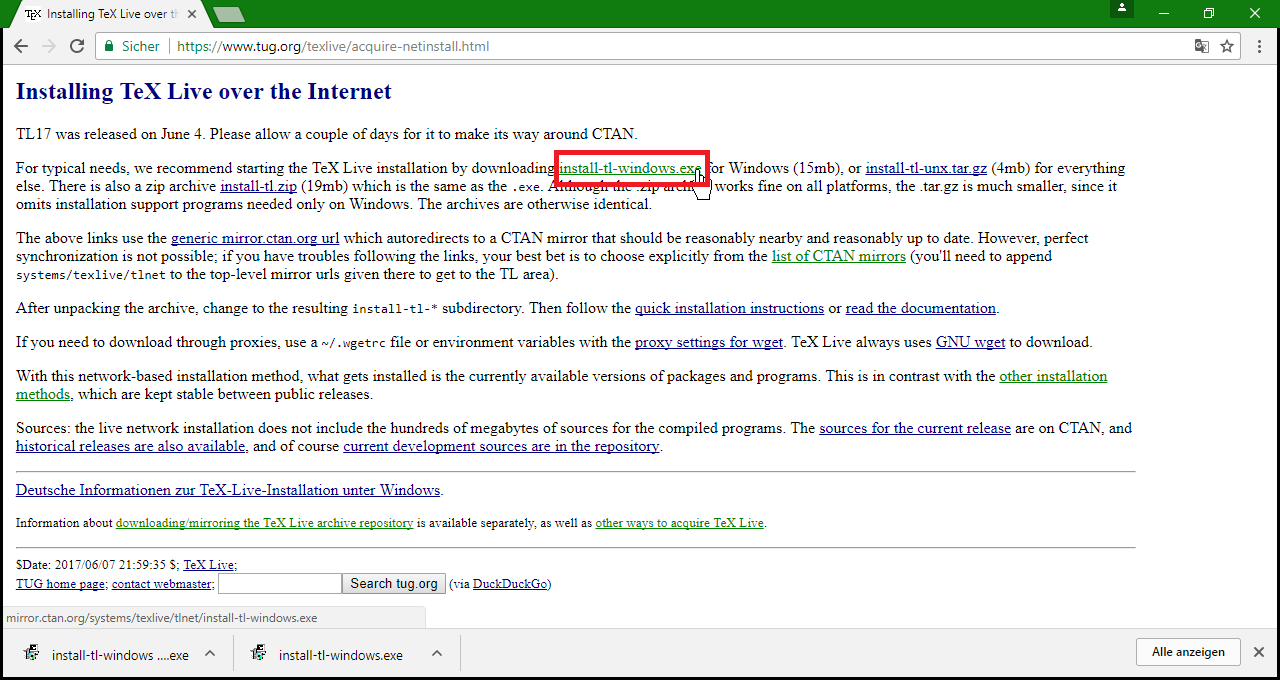
\includegraphics[width=\textwidth]{windows/p2.png}
\end{figure}
%\end{minipage}
\FloatBarrier

\section*{Schrittweise:}
%\begin{minipage}[t]{\textwidth}

\noindent
\begin{minipage}[c]{\textwidth}
\centering
\captionof{figure}{Führe den Installer als Administrator aus. }
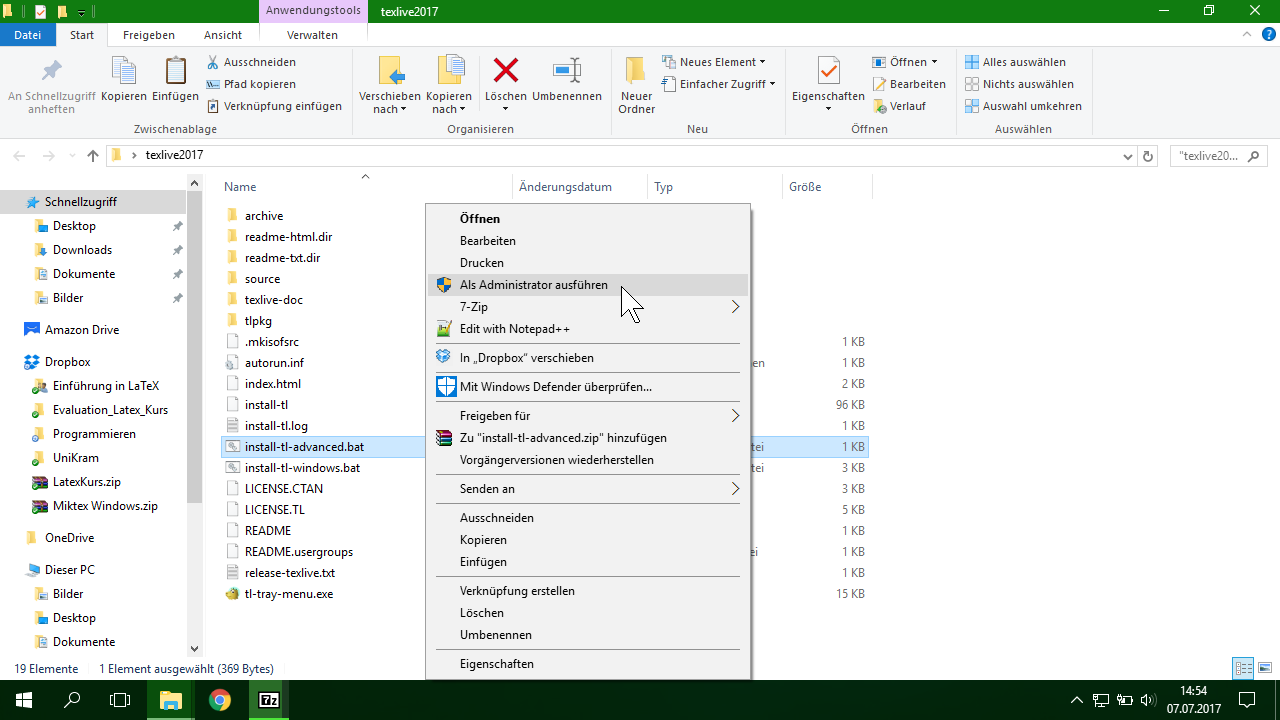
\includegraphics[width=\textwidth]{windows/p3.png}
\\~\\
\captionof{figure}{Führe den Installer aus und wähle bei weitere Einstellungen ändern aus. }
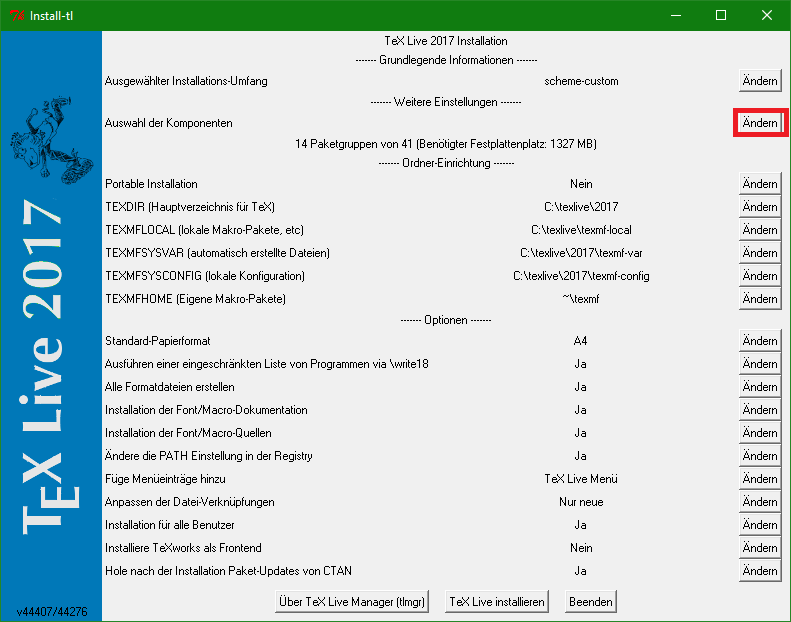
\includegraphics[width=.8\textwidth]{windows/p4.png}
\end{minipage}
\FloatBarrier



\noindent
\begin{minipage}[c]{\textwidth}
\centering
\captionof{figure}{Wähle die folgenden Komponenten aus. Diese brauchen ca. 2,1 GB Speicherplatz.}
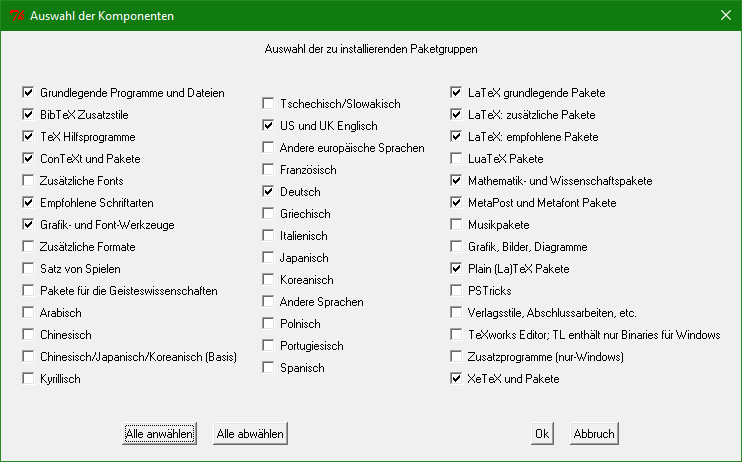
\includegraphics[width=.9\textwidth]{windows/p5.png}
\\~\\~\\
\captionof{figure}{Tex Live wird jetzt installiert.}
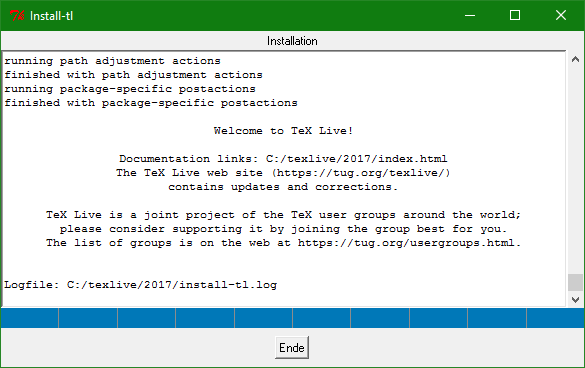
\includegraphics[width=.9\textwidth]{windows/p6.png}
\end{minipage}
\FloatBarrier



\noindent
\begin{minipage}[c]{\textwidth}
\centering
\captionof{figure}{Nun musst du noch Texmaker von \url{http://www.xm1math.net/texmaker/download.html} herunterladen und installieren.}
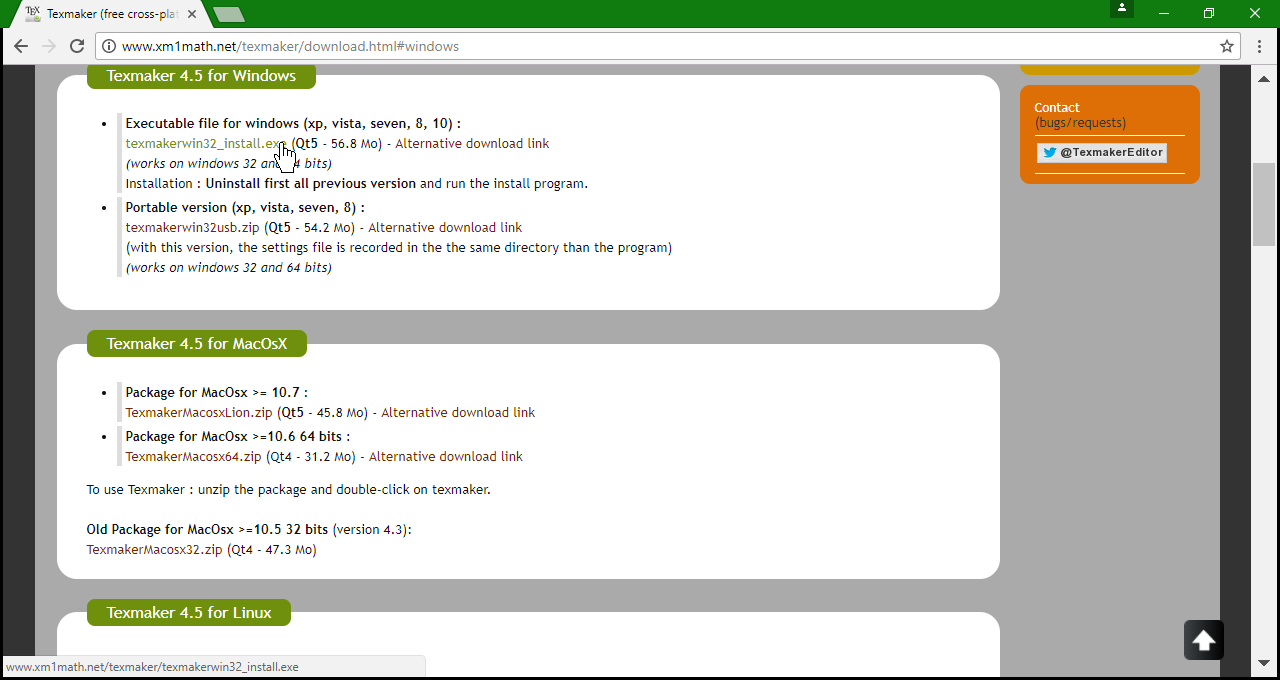
\includegraphics[width=\textwidth]{windows/texmaker1.png}
\\~\\~\\
\captionof{figure}{Starte jetzt Texmaker und gehe auf Optionen>Texmaker konfigurieren}
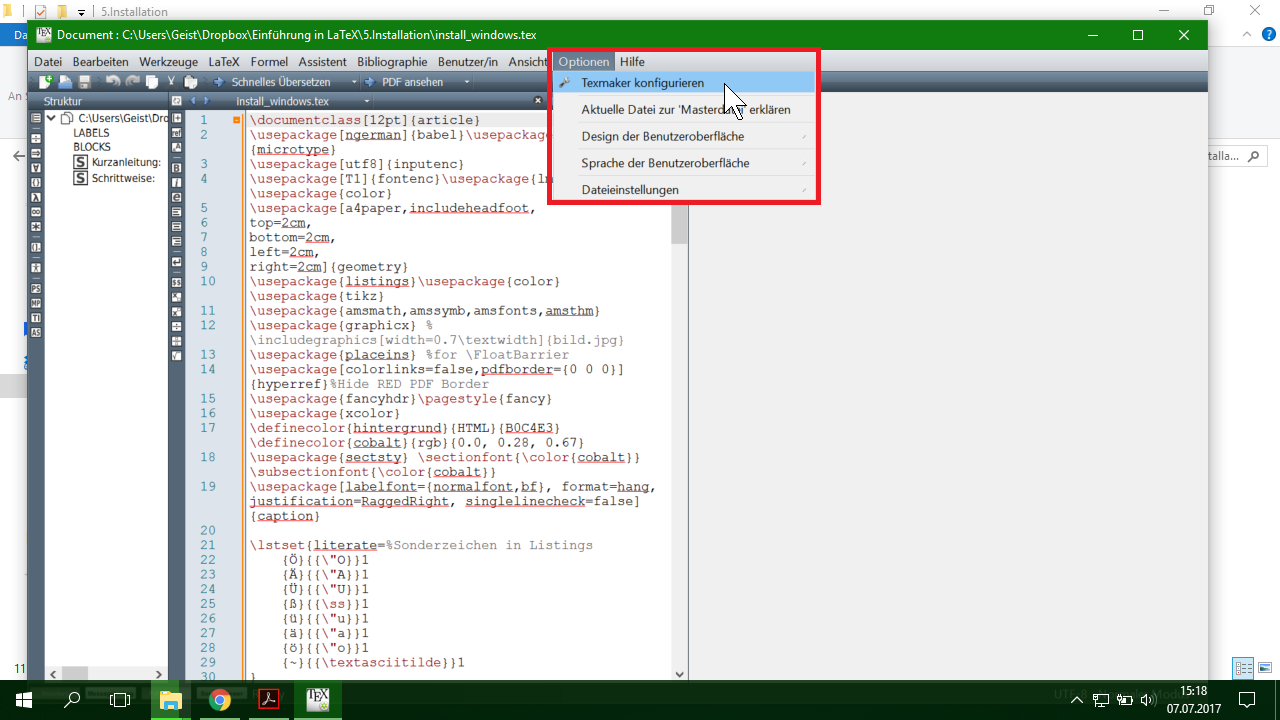
\includegraphics[width=\textwidth]{windows/texmaker2.png}
\end{minipage}


\noindent
\begin{minipage}[c]{\textwidth}
\centering
\captionof{figure}{Mache einen Haken bei Unterordner ''build'' für die Ausgabe nutzen.}
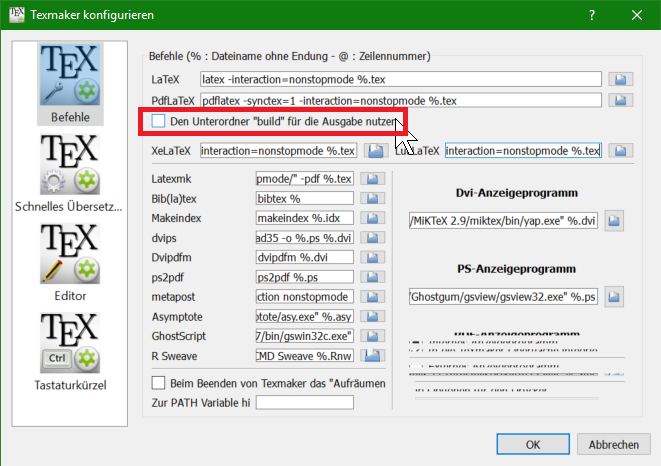
\includegraphics[width=.9\textwidth]{windows/texmaker3.png}
\\~\\~\\
\captionof{figure}{Erstelle dein erstes \LaTeX Dokument}
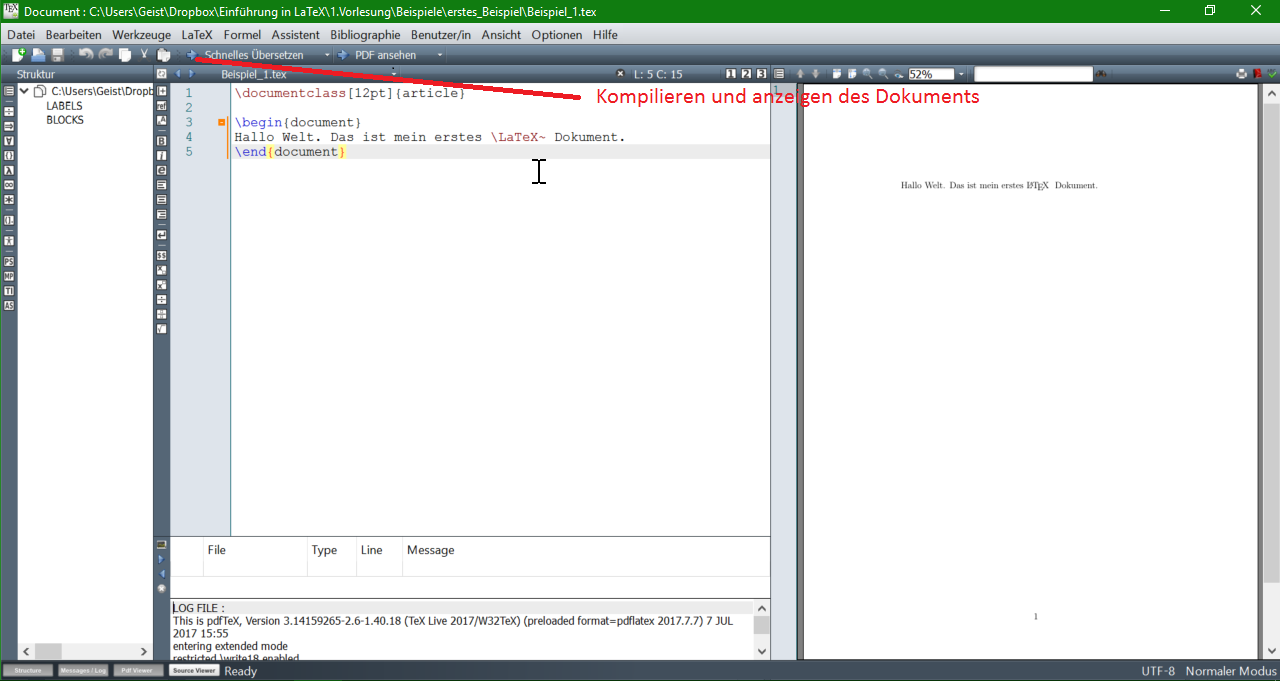
\includegraphics[width=\textwidth]{windows/texmaker5.png}
\end{minipage}


\begin{center}
Gratulation! Du hast nun eine verwendbare LaTeX-Installation.
\end{center}
\FloatBarrier
\end{document}